\subsection{Генетический алгоритм}
\label{sec:1c}

Использование генетического алгоритма для оптимизации кластерных структур
началось в 90-х годах с работ Хартке (для кремниевых кластеров малого размера)
\cite{hartke} и Вильямса (для молекулярных кластеров) \cite{williams}. В обоих
случаях структура кластеров была закодирована с помощью бинарных строк. При этом
генетические операторы использовали бинарные операции над ними. Важным улучшением
генетического алгоритма для кластерной оптимизации стало использование действительных
Декартовых координат для представления кластеров. Этот подход был предложен
Зейри \cite{zeiri} и позволил снять ограничение на бинарное кодирование генов.

Следующий шаг в развитии генетических алгоритмов для кластерной оптимизации был
предложен Дивеном и Хо \cite{deaven}. Главной идеей является нахождение локального
минимума общей потенциальной энергии кластера для каждого кластера, полученного
с помощью генетического алгоритма на очередном шаге. Это позволяет значительно
уменьшить пространство возможных решений для генетического алгоритма.

Дивен и Хо также предложили трехмерный оператор скрещивания, которую назвали
"разрез и склеивание" ("cut and splice"). Этот оператор, который использовался
в большинстве последующих работ по кластерной оптимизации, привносит больше 
физического значения в процесс скрещивания. Этот механизм будет описан более
подробно позже.

На основе вышеперечисленных разработок в области генетических алгоритмов для
кластерной оптимизации Джонстон и др. предложили генетический алгоритм,
который назвали "Бирмингемским" \cite{johnston}. Именно этот алгоритм и был
выбран при реализации экспериментального программного обеспечения.
Основные особенности этого алгоритма описаны ниже:

{\it Инициализация}.  % TODO: not generated, but initialized with initial cluster state? add more to generation if random
Для кластера заданного размера (состоящего из $N$ элементов) генерируется $N_{clus}$
(значение по умолчанию - 20) кластеров случайным образом для формирования начальной
популяцию.

{\it Функция приспособленности}

Функция приспособленности конкретной особи это оценка качества особи с точки зрения
конкретной задачи. В данном случае, кластеры с наименьшей энергией (наименьшей $V_{clus}$)
имеют наибольшее значение функции приспособленности. Генетический алгоритм использует
динамическое масштабирование приспособленности, основанное на нормализованном значении
энергии, $\rho$:

\begin{equation}
  \rho_{i} = \frac{V_{i} - V_{min}}{V_{max}-V_{min}}
\end{equation}

где $V_{min}$ и $V_{max}$ минимальное и максимальное значение энергии кластеров в
текущей популяции соответственно.

{\bf Скрещивание}

Родители для скрещивания выбираются с помощью "турнирного" метода. Несколько кластеров
выбираются случайным образом, чтобы образовать "турнирную" группу. Два кластера с минимальной
энергией затем выбираются из этой группы в качестве родителей. При такой схеме кластеры
с наибольшим значением функции приспособленности имеют высокую вероятность быть выбранными
для скрещивания и таким образом передать особенности своей структуры следующим поколениям.

Используемая процедура скрещивания представляет собой вариант оператора "разрез и склеивание",
предложенного Дивеном и Хо \cite{deaven}. К кластерным структурам обоих родителей сначала
применяются случайные повороты вокруг двух перпендикулярных осей, а затем оба кластера разрезаются
горизонтально параллельно плоскости $xy$ посередине и соответствующие части склеиваются вместе,
как показано на рис. \ref{cut_and_splice}.

В результате процедуры скрещивания появляется один новый потомок. "Турнирный метод" применяется
столько раз, сколько потомков необходимо получить в следующем поколении.
Для каждый кластера-потомка затем применяется градиентный метод, чтобы структура кластера
соответствовала ближайшему локальному минимуму потенциальной энергии.

\begin{figure}[h!]
\centering
  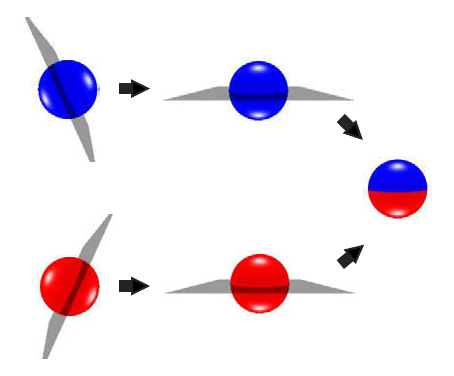
\includegraphics[width=0.5\textwidth]{./FIGs/cut_and_splice.png}
\caption{Оператор скрещивания "разрез и склеивание"}
\label{cut_and_splice}
\end{figure}

{\bf Мутация}

Несмотря на то, что операция скрещивания приводит к перемешиванию генетического материала
в кластерах-потомках, нового генетического материала при этом не появляется. Для того, чтобы
поддержать разнообразие особей в популяции, вводится новый оператор мутации. Каждая особь
имеет некоторую вероятность подвергнуться мутации ($P_{mut}$), которая возмущает некоторые или
все позиции атомов внутри кластера. После мутации, каждая особь локально минимизируется.

Может быть использовано несколько видов мутации:

\begin{itemize}
  \item{\bf Перемещение атомов} {Данная мутация заменяет координаты некоторых атомов кластера
случайными значениями. Количество атомов для замены координат было выбрано равным
трети ($N/3$) от общего количества атомов.}
\item{\bf Вращение} Происходит поворот верхней части кластера вокруг оси $z$ на случайный угол
относительно нижней части кластера.
\item{\bf Замена кластера} Происходит замена целого кластера на новый, координаты которого заданы
случайным образом. 
\end{itemize}

Перечисленные мутации приводят к достаточно значительным изменениям генетического материала.


{\bf Последующие популяции}

Новая популяция представляет собой объединение некоторого количества ($N_{clus}$) кластеров
с большими значениями функции приспособленности, некоторого количества потомков ($N_{off}$),
а также некоторого количества мутировавших кластеров.

Процесс последовательного скрещивания, мутации и селекции происходит заданное количество
раз ($N_{gen}$).
